\chapter{Detector Design and Construction Organization}
\label{vl:tc-overview}

The design and construction of the \dword{dune} detector elements is 
carried out by the international \dword{dune} Project.  \dword{dune}
Collaboration management is responsible for overseeing this portion 
of the global project and ensuring its successful execution.  
The high-level dword{dune} management team consisting of the 
co-spokespersons, \dword{tcoord}, and \dword{rcoord} is responsible 
for the day-to-day administration of the project.  

\section{\dword{dune} Work Flow}
\label{sec:workflow}

Figure~\ref{fig:DUNE_workflow} indicates the time-sequenced set of 
activities needed to implement the \dword{dune} far detector modules.
The \dword{dune} project has direct responsibility for the design, 
prototyping, fabrication, and transportation of the far detector 
elements.  These activities are managed by the \dword{dune} \dword{tc} 
organization under the direction of the \dword{tcoord}.  Activities at 
or in the vicinity of SURF are managed by the on-site integration and
installation team under the direction of the \dword{ipd} as described 
in Chapter~\label{ch:tc-jpo}.  These activities include the receipt,
processing, installation, and operation of the detector components.            
\begin{dunefigure}[\dword{dune} work flow]{fig:DUNE_workflow}
  {\dword{dune} work flow.}
  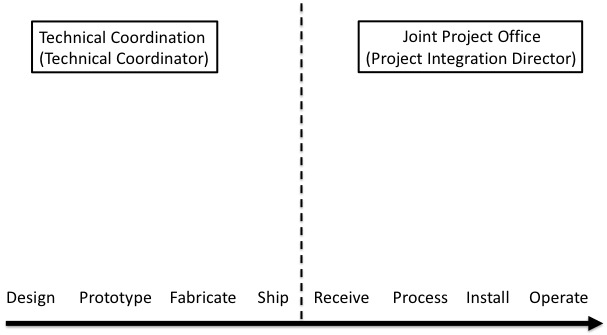
\includegraphics[width=0.99\textwidth]{DUNE_workflow}
\end{dunefigure}

Although responsibilities for the two sets of time-ordered activities 
are clearly delineated, both management teams have roles in supporting
the activities that do not fall under their direct responsibility.  The 
integration and installation team interacts directly with the \dword{dune} 
project team through detector design, prototyping, and construction to 
ensure that fabricated detector elements are properly integrated within 
the supporting infrastructure.  Conversely, the \dword{dune} project 
supports the integration and installation activies at SURF by providing 
some of the dedicated resources (both personnel and equipment) necessary 
for carrying out these activities.  Ensuring proper installation and 
commissioning of the detector elements remains a \dword{dune} project
responsibility even while the global coordination of integration and 
installation activities is managed through the on-site organization.  

The \dword{dune} project has already completed an initial round of design 
and prototyping activities culminating in the construction and operation 
of the \dword{protodune} detectors.  Moving forward, the project is 
updating detector component designs to account for lessons-learned from 
the \dword{protodune} experience.  Upon finalization of the designs, the 
project will construct first production versions of all components, which 
will be installed and operated in a second phase of \dword{protodune} 
operations prior to the start of full-scale production.  The operation 
of the \dword{protodune2} detectors will follow roughly two years after
the end of operations for the corresponding \dword{protodune} detectors.
In a few cases, the production of long lead-time components will need to 
be started in parallel with the operation of first production components 
in \dword{protodune2}.

\section{\dword{dune} Consortia}
\label{sec:consortia}

Construction of the \dword{dune} far \dwords{detmodule} is carried out by 
``consortia of collaboration institutions'' who assume responsibility for 
detector subsystems.  Each consortium plans and executes the construction, 
installation and commissioning of its subsystem.

Management of the consortia is through an overall Consortium Leader and 
a Technical Lead.  The Consortium Leader chairs an institutional board 
composed of one representative from each of the collaboration institutes 
contributing to the activities of the consortium.  Major consortia decisions 
such as technology selections and assignment of responsibilities within 
the institutions are expected to be passed through its Institutional Board.  
These decisions are then passed as recommendation to the \dword{dune} 
\dword{exb}, as described in greater detail below, for formal collaboration 
approval.

Figure~\ref{fig:DUNE_consortia_org} shows an example consortia organizational 
chart with the different parts of the internal consortia structure mandated 
by \dword{dune} Collaboration management.  In addition to the pieces described 
above, the consortium in most cases needs to manage sub-system deliverables 
that are supported by more than a single funding agency.  In the example case 
illustrated here, responsibilities for sub-system deliverables are shared 
between the United States, United Kingdom, and Switzerland, where each of the 
funding agencies is expected to manage their own internal projects which have
direct responsibility for their assigned deliverables.  To ensure coordination
between the separate internal projects contributing to the consortium, the 
Technical Lead is responsible for chairing a consortium Project Management 
Board incorporating the separate managers from each of the internal projects.   
\begin{dunefigure}[\dword{dune} Internal Consortia Structure]{fig:DUNE_consortia_org}
  {\dword{dune} Internal Consortia Structure}
  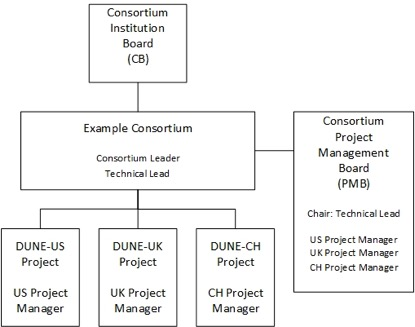
\includegraphics[width=0.99\textwidth]{DUNE_consortia_org}
\end{dunefigure}

In addition to the mandated organizational pieces described here, the consortia 
incorporate additional internal structures as needed to deliver their assigned 
sub-systems.  For example, working groups with convenors are typically appointed 
to focus on specific consortia activities, and steering committees are in many 
cases formed to help guide technical and strategic decisions within the consortia.
Each consortia is also expected to appoint both safety and quality assurance  
representatives as well as a representative with responsibility for integration 
and installation issues.  These individuals are charged with interacting directly 
with appropriate project management team personnel to ensure proper coordination 
on these topics across the consortia.        

\section{\dword{dune} Collaboration Management}
\label{sec:dune_mgmt}

The high-level \dword{dune} collaboration management structure is shown 
in Figure~\ref{fig:DUNE_org}.  The \dword{dune} \dword{exb} is the primary
collaboration decision-making body and as such includes representatives 
from all major areas of activity within the collaboration.
\begin{dunefigure}[\dword{dune} org chart]{fig:DUNE_org}
  {\dword{dune} Organizational Chart}
  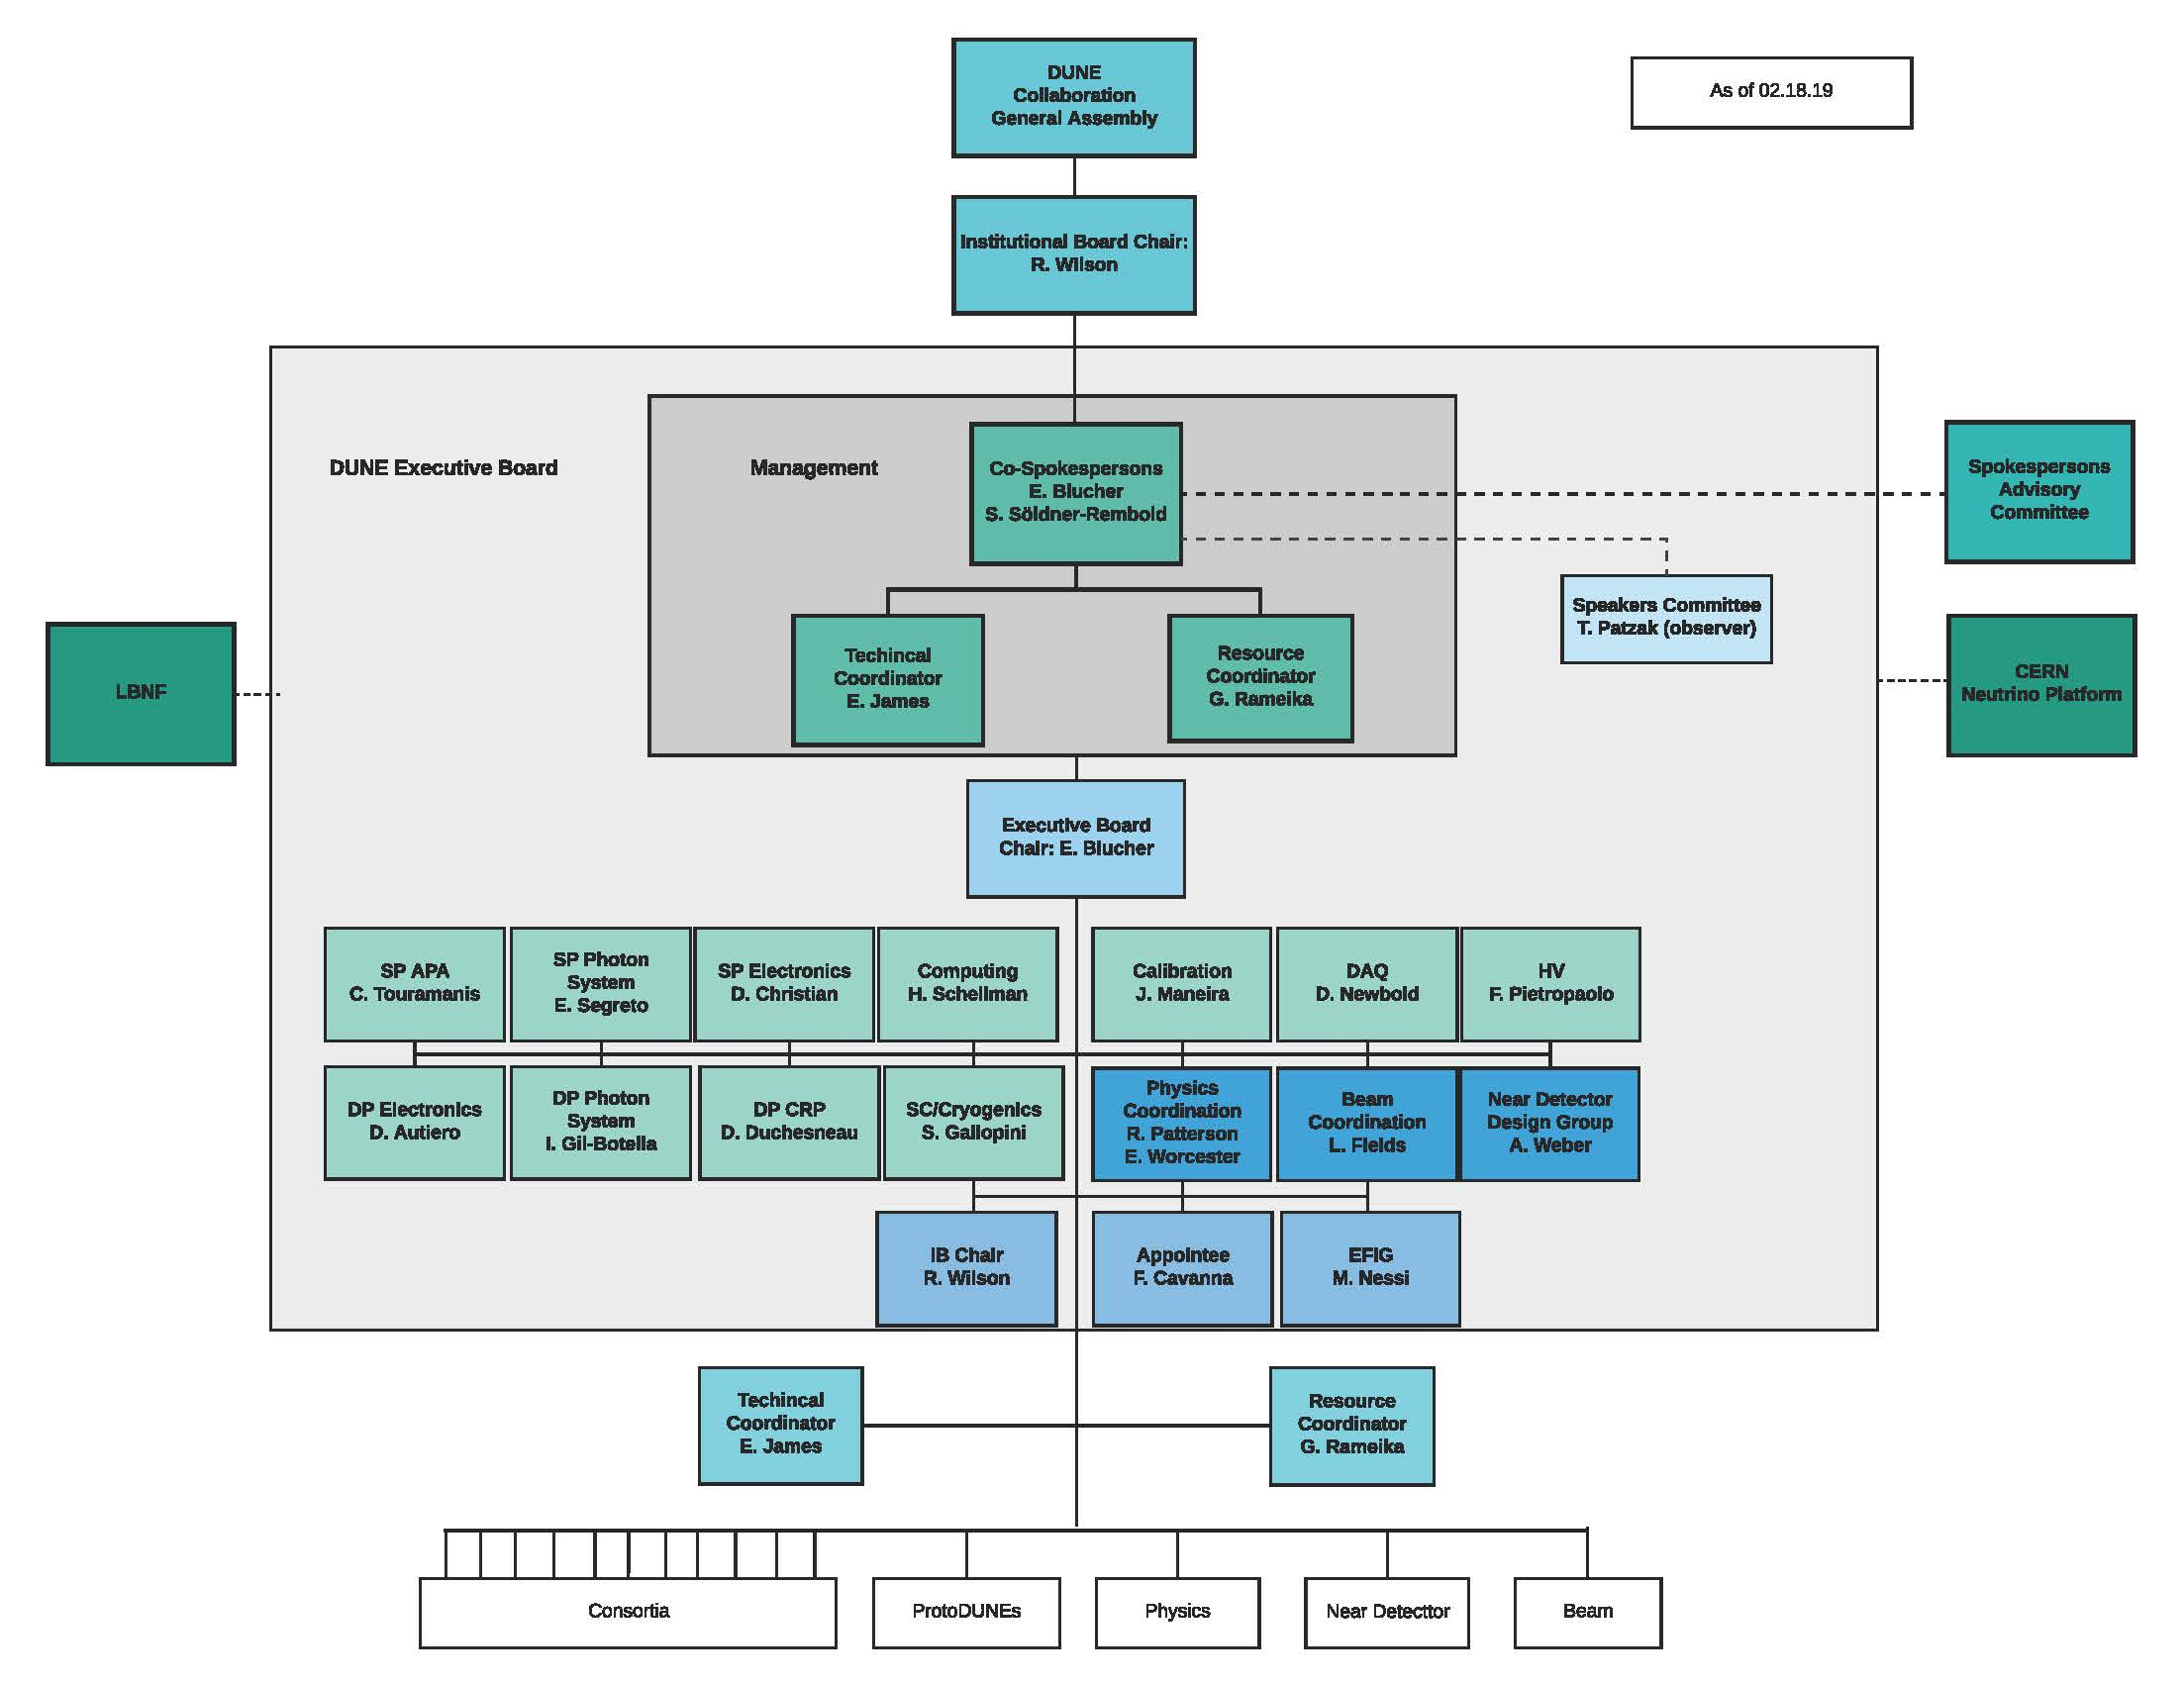
\includegraphics[width=0.99\textwidth]{DUNE_COllab_Mgmt}
\end{dunefigure}

Each of the consortia is represented on the \dword{dune} \dword{exb} by its 
consortium leader.  All collaboration decisions, especially those with potential 
impacts on the \dword{dune} scientific program or connected with the assignment 
of institutional responsibilities, pass through the \dword{exb}.  \dword{exb} 
decisions are expected to be achieved through consensus.  In cases where consensus 
cannot be obtained, decision-making responsibility passes to the co-spokespersons.

\section{\dword{tc}}
\label{sec:tc}

Because the consortia operate as self-managed entities, a strong
\dword{tc} organization is required to ensure overall integration 
of the detector elements and successful execution of the detector
construction project.  \dword{tc} areas of responsibility include 
general project oversight, systems engineering, quality assurance 
and safety.  In association with the support role provided by 
the consortia, \dword{tc} also works closely with the on-site 
team responsible for planning and executing the required 
detector integration and installation activities in the nearby 
surface facilities and underground detector caverns at \surf 
(see Chapter~\label{ch:tc-jpo}).  

\dword{tc} is headed by the \dword{tcoord}, who is an \dword{fnal}
employee and is appointed jointly by the \dword{fnal} director and 
the \dword{dune} co-spokespersons.  A deputy technical coordinator 
is selected from within the collaboration to assist the \dword{tc} 
in carrying out their responsibilities.

The \dword{tcoord} manages the overall detector construction project
through regular board meetings with the consortia leadership teams and 
members of the \dword{tc} organization (see Section~\label{sec:tco}).  
These board meetings are used to identify and resolve technical issues
and serve as the primary forums for required interactions between the 
consortia leadership teams.

Technical Board meetings are used to evaluate consortia design
decisions with potential impacts on overall detector performance,
ensure that interfaces between the different subsystems are well
understood and documented, and monitor the overall construction
project to identify and address both technical and interface issues 
as they arise.

Project board meetings are used to ensure that the scopes of each
consortium are fully documented with assigned institutional
responsibilities, develop and manage risks held within a global
project registry, review and manage project change requests, and
monitor the status of the overall detector construction schedule.

Any decisions generated through these board meetings are passed to 
the \dword{dune} \dword{exb} as recommendations for formal approval.
Depending on the agenda items to be discussed at a specific board 
meeting, the \dword{tcoord} will invite additional members of the 
collaboration with specific knowledge or particular expertise to 
participate.  In addition, for major decisions, the \dword{tcoord} 
will officially appoint three internal collaboration referees with 
no direct conflicts of interest to directly engage in the process.

\section{\dword{tc} Organization}
\label{sec:tco}

The \dword{tcoord} heads an organization that supports the work of 
the consortia and has responsibility for a number of major project 
support functions including

\begin{itemize}
\item Ensuring that each consortium has a well defined and complete
  scope, that interactions between the consortia are sufficiently 
  well defined, and that any required scope sitting outside of the 
  consortia is provided through other sources such as collaboration
  common funds.
\item Defining and documenting scope boundaries and technical 
  interfaces both between the consortia and with \dword{lbnf}.  
\item Developing an overall schedule with appropriate dependencies
  between activities covering all phases of the project 
\item Ensuring that appropriate engineering and safety standards 
  are developed, understood, and agreed to by all key stakeholders 
  and that these standards are conveyed to and understood by each
   of the consortia.
\item Ensuring that all \dword{dune} requirements on \dword{lbnf} 
  for conventional facilities, cryostat and cryogenics are clearly
  defined and agreed to by each consortium.
\item Ensuring that each consortium has well developed and reviewed
  component designs, constrution plans, \dword{qc} processes, and 
  safety programs.
\item Monitoring of the overall project schedule and the progress 
  of each consortium towards deliving its assigned scope. 
\end{itemize}
 
\begin{dunefigure}[\dword{dune} \dword{tc} org chart]{fig:DUNE_tc}
  {\dword{dune} \dword{tc} Organizational Chart}
  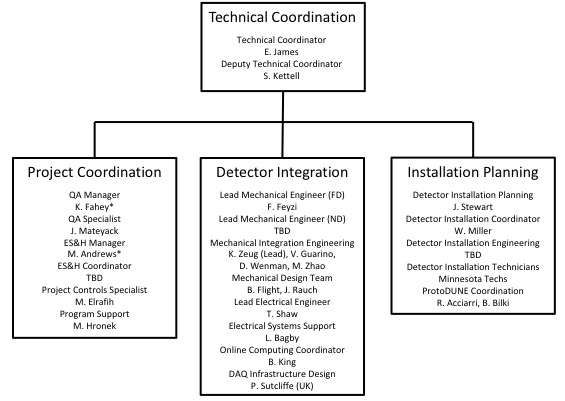
\includegraphics[width=0.99\textwidth]{DUNE_tc}
\end{dunefigure}

The \dword{dune} \dword{tc} organizational structure is shown in 
Figure~\ref{fig:DUNE_tc}.  The strcuture incorporates teams with 
responsibilities towards project coordination, detector integration,
and installation support.  Many of the \dword{tc} also sit within 
the \dword{jpo} team shown in Figure\ref{fig:jpoOrg} that ensures 
coherency in these activities across the global project.

The project coordination team is led by a lead project controls
specialist, a \dword{qa} manager and an \dword{esh} manager.  The
detector integration team is directed by a lead mechanical and lead
electrical engineer, and inorporates an online computing coordinator.
The installation support team is headed by the planning coordinators 
for activities associated with the integration and installation of 
detector components in the underground areas.  Each of the three 
teams incorporates additional personnel to support these individuals 
in carrying out their areas of responsibility.  Members of the 
/dword{tc} organization meet weekly to review project progress and 
discuss detailed technical issues. 
     
Within the context of the \dword{dune} project, \dword{tc} functions 
associated with its coordination role include

\subsection{Safety}

\subsection{Engineering Integration (CAD Models, Drawings, Interfaces, Mechanical \& Electrical)}

\subsection{Change Control and Document Management (Requirements, Quality Assurance Database)}

\Dword{tc} maintains a web
page\footnote{\url{https://web.fnal.gov/collaboration/DUNE/DUNE\%20Project/\_layouts/15/start.aspx\#/}.}
with links to project documents. \Dword{tc} also maintains repositories of project documents and drawings.
These include the \dword{wbs}, schedule, risk register, requirements, milestones, strategy, detector 
models and drawings that define the \dword{dune} detector.

\subsection{Schedule and Milestones}

\subsection{Review Process}

\subsection{Partner Agreements and Financial Reporting}








